%\documentclass[a4paper,fleqn,longmktitle]{cas-sc}
\documentclass[a4paper,fleqn]{cas-sc}
\usepackage[utf8]{inputenc}
\DeclareUnicodeCharacter{0131}{\i}
\DeclareUnicodeCharacter{0301}{\'{}}
\usepackage{siunitx}
%\usepackage[numbers]{natbib}
\usepackage{natbib}
\usepackage{placeins}
\usepackage{url}
\usepackage{graphicx}
\usepackage{makecell}
\usepackage[T1]{fontenc}
\usepackage{parskip}
\usepackage{amsmath}
%\usepackage[spanish]{babel}
%\selectlanguage{spanish}
\usepackage[utf8]{inputenc}
\usepackage{hyperref}
\usepackage{lineno}
% Visible revision markup
\usepackage{xcolor}
\usepackage[normalem]{ulem}
\DeclareRobustCommand{\deleted}[1]{\textcolor{red}{\sout{#1}}}
\DeclareRobustCommand{\added}[1]{\textcolor{blue}{#1}}


%%%Author definitions
\def\tsc#1{\csdef{#1}{\textsc{\lowercase{#1}}\xspace}}
\tsc{WGM}
\tsc{QE}
\tsc{EP}
\tsc{PMS}
\tsc{BEC}
\tsc{DE}

% Uncomment and use as if needed
%\newtheorem{theorem}{Theorem}
%\newtheorem{lemma}[theorem]{Lemma}
%\newdefinition{rmk}{Remark}
%\newproof{pf}{Proof}
%\newproof{pot}{Proof of Theorem \ref{thm}}

\begin{document}
\linenumbers
\let\WriteBookmarks\relax
\def\floatpagepagefraction{1}
\def\textpagefraction{.001}

% Short title
\shorttitle{28 years of macroalgae diversity shifts in the Canary Islands}

% Short author
\shortauthors{Geppi et~al.}

% Main title of the paper
\title [mode = title]{Spatiotemporal patterns of macroalgal diversity across an environmentally heterogeneous oceanic archipelago}    

\author[1]{Eros Fernando Geppi}
\author[2]{Daniel Gonzalez-Aragon}
\author[1]{Rodrigo Riera \corref{corr}}


\affiliation[1]{organization={Grupo en Biodiversidad y Conservación, IU-ECOAQUA, Universidad de Las Palmas de Gran Canaria, Marine Scientific and Technological Park, Crta. Taliarte s/n, 35214 Telde, Spain}}
\affiliation[2]{organization={Departamento de Ecología, Facultad de Ciencias, Universidad Católica de la Santísima Concepción, Chile}}


% Corresponding author text
\cortext[corr]{Corresponding author: Rodrigo Riera (\href{https://orcid.org/0000-0003-1264-1625}{ORCID: 0000-0003-1264-1625})}
\ead{rodrigo.riera@ulpgc.es}


\begin{abstract}
Anthropogenic climate change is altering oceanographic conditions worldwide, with particularly strong implications for coastal ecosystems and habitat-forming macroalgae. Detecting long-term patterns in macroalgal diversity under environmental variability remains challenging, especially in regions characterized by strong spatial heterogeneity. Here, we integrate nearly three decades of macroalgal occurrence records with satellite-derived environmental data to examine spatiotemporal patterns of macroalgal diversity across the Canary Islands (NE Atlantic). Using historical biodiversity records spanning 1993-2023,  we quantified alpha, beta, and gamma diversity at island and regional scales. We subsequently related these patterns to physical and biogeochemical variables derived from the Copernicus Marine Environment Monitoring Service. Spatial patterns were evaluated along the pronounced east-west environmental gradient of the archipelago, while temporal trends were assessed across seasonal, interannual, and decadal scales. Relationships between macroalgal diversity and environmental variability were explored using generalized additive models and multivariate analyses. Macroalgal diversity exhibited strong spatial structuring across islands. Eastern islands, influenced by cooler and nutrient-enriched waters, and western islands, characterized by warmer and more oligotrophic conditions, showed contrasting diversity patterns and community compositions.
Beta diversity analyses revealed clear compositional clustering among islands, consistent with regional environmental differentiation. Temporally, species richness increased during the 2000s but declined in subsequent decades, particularly in western islands, against a background of coherent inter-decadal changes in oceanographic conditions. Statistical models indicated that macroalgal diversity metrics were associated with multiple environmental variables through non-linear relationships. Model performance improved when analyses were stratified by region rather than conducted at the archipelago-wide scale. These patterns are compatible with a gradual reorganization of macroalgal communities under long-term environmental variability, although causal mechanisms cannot be directly inferred from the observational data. By combining long-term biological records with satellite-derived environmental information, this study provides a regional-scale baseline of macroalgal diversity dynamics in an environmentally heterogeneous archipelago. The results highlight the importance of spatial context and scale when assessing biodiversity responses to contemporary climate variability and offer a framework for future macro-ecological analyses in coastal systems.
\end{abstract}

\begin{highlights}
\item Macroalgal diversity followed an east-west environmental gradient.
\item Richness increased in the 2000s and declined afterwards.
\item Western islands showed the strongest recent richness declines.
\item Diversity-environment links were non-linear and scale-dependent.
\item Occurrence records and satellite data provide a regional baseline.
\end{highlights}

\begin{keywords} coastal ecosystems, marine biodiversity gradients, community composition, environmental heterogeneity, satellite oceanography, macro-ecological patterns.
\end{keywords}

\maketitle

\section{Introduction}
Anthropogenic climate change is altering marine environments through sustained increases in sea surface temperature, modifications of circulation patterns, and changes in water column stratification, with profound consequences for coastal ecosystems \citep{SANGIL2012, Doneyetal2012, ANI202, Huang2024}. These changes are particularly critical in shallow coastal systems, where benthic communities experience rapid exposure to thermal stress, nutrient variability, and hydrodynamic forcing \citep{Noissetteetal2022}. As a result, many marine species undergo range changes, local population declines, or compositional reorganization when environmental thresholds are exceeded \citep{Belsega2013, Assan2020, Gianluigietal2021}.

Habitat-forming macroalgae represent one of the most sensitive and ecologically consequential components of coastal ecosystems under environmental change \citep{Ji2021, Noissetteetal2022}. These taxa play a central role in structuring benthic habitats, sustaining trophic interactions, and supporting ecosystem services such as fisheries production and coastal protection \citep{RILOV2020105045, Nahor2024}. Documented responses of macroalgal communities to environmental change include distributional shifts, local extinctions, and changes in dominance patterns, often accompanied by increases in opportunistic or warm-affinity species \citep{SANGIL2012, Vergesetal2016, JI202191}. Understanding how macroalgal diversity responds to long-term environmental variability is therefore essential for anticipating future ecosystem trajectories under ongoing ocean warming. Long-term ecological records provide a valuable opportunity to assess biodiversity response across decadal timescales. In marine systems, historical herbarium collections and biodiversity databases can capture temporal and spatial patterns that are otherwise difficult to detect through short-term field studies \citep{Lang2019, Antao2020}. When combined with satellite-derived oceanographic data, these records enable macro-ecological analyses that integrate biological patterns with environmental variability across broad spatial and temporal scales \citep{Duffy2019Toward}. Such integrative approaches are increasingly used to identify persistent signals associated with climate variability while accounting for natural interannual fluctuations \citep{Mahmoud2025}.

The Canary archipelago constitutes a particularly suitable natural laboratory for examining long-term macroalgal diversity patterns in an environmentally heterogeneous setting. Located within the upwelling system of the Canary Current, the archipelago is characterized by a pronounced east-west environmental gradient driven by differential exposure to coastal upwelling from northwest Africa \citep{Barton1998, Aristegui2009, Barton2016}. The eastern islands are influenced by cooler and nutrient-rich waters, while the western islands experience warmer, more oligotrophic conditions and greater stability of the water column. Previous studies have shown that this gradient shapes the composition of marine communities in multiple taxa, including macroalgae, fish, and invertebrates \citep{Barton1998, SANGIL2012, Valdazoetal2017}. In addition to its strong environmental gradients, the Canary Islands host high levels of marine biodiversity and endemism and benefit from extensive historical biodiversity records that span several decades \citep{RIERA2015}. From a macro-ecological perspective, macroalgal assemblages in the archipelago can be viewed as spatially structured systems in which local diversity patterns are embedded within broad regional environmental gradients \citep{Duffy2019Toward}. In such contexts, persistent differences in oceanographic conditions may modulate alpha diversity at the island scale, species turnover among islands, and temporal variability in regional diversity \citep{RILOV2020105045}. Assessing these patterns requires analytical approaches that explicitly consider spatial heterogeneity, scale dependence, and the observational nature of long-term biodiversity data \citep{Medrano2019Long-term}.

In this study, we integrate nearly three decades of macroalgal occurrence records with satellite-derived oceanographic data to examine spatiotemporal patterns in macroalgal diversity across the Canary Islands. Specifically, we aim to characterize spatial patterns of alpha and beta diversity among islands in relation to the east-west environmental gradient described for the Canary Current upwelling system \citep{Barton1998, Aristegui2009, Barton2016}, assess temporal variability and long-term trends in island-level and regional macroalgal diversity across seasonal to decadal scales, and evaluate associations between macroalgal diversity metrics and environmental variability using multivariate analyses and generalized additive models (GAMs).

We hypothesized that macroalgal diversity would be spatially structured along the archipelago's pronounced east-west environmental gradient, with differences between eastern islands, influenced by cooler, nutrient-enriched waters, and western islands, characterized by warmer, more oligotrophic conditions \citep{Barton1998, Aristegui2009, Barton2016}. We further expected temporal changes in diversity to be associated with long-term variability in physical and biogeochemical drivers linked to contemporary anthropogenic climate change, including sea surface temperature, stratification-related variables, nutrient availability, dissolved oxygen, and surface $C0_{2}$ conditions.Finally, following a macro-ecological perspective for broad-scale marine biodiversity assessment \citep{Duffy2019Toward}, we hypothesized that the diversity-environment relationship would be non-linear and scale-dependent, with regional models better capturing ecological patterns than a single archipelago-wide model.

By adopting a macro-ecological perspective grounded in long-term observational data \citep{Duffy2019Toward}, this study provides a regional-scale baseline for understanding how environmentally heterogeneous coastal systems respond to sustained environmental variability under ongoing climate change. Our results offer insights relevant for biodiversity assessment and contribute to broader discussions of the role of spatial context and scale in evaluating ecological responses to contemporary climate variability in marine environments.



\section{Methods}
\subsection{Study area}
This study was conducted in the Canary archipelago, located in the northeast Atlantic Ocean off the northwest coast of Africa. The archipelago comprises seven main islands (El Hierro, La Palma, La Gomera, Tenerife, Gran Canaria, Fuerteventura, and Lanzarote) that exhibit pronounced environmental heterogeneity due to their volcanic origin, oceanic setting, and exposure to the Canary Current system \citep{Barton1998}. A key feature of the region is a strong east-west environmental gradient driven by differential exposure to coastal upwelling off northwest Africa, which generates persistent spatial contrast in oceanographic conditions across the archipelago \citep{Aristegui2009}.

Based on this oceanographic context, islands were grouped into two biogeographic subregions for analytical purposes. The western group (El Hierro, La Palma, La Gomera, and Tenerife) is characterized by warmer, more oligotrophic waters and relatively stable oceanographic conditions, whereas the eastern group (Gran Canaria, Fuerteventura, and Lanzarote) is influenced by cooler, nutrient-enriched waters associated with upwelling processes \citep{Aristegui2009, Bianchi2012}. This regional classification provided a consistent spatial framework for exploring differences in macroalgal diversity and its relationships with environmental variability \citep{Duffy2019Toward}.

\subsection{Macroalgae records}

Macroalgal occurrence records were compiled from herbarium collections and institutional biodiversity databases, primarily the Canary Islands Biodiversity Data Bank (CIBDB) \citep{RIERA2015}. The dataset spans approximately three decades (1993-2023) and includes taxonomic identification at the species level, collection date (year and month), and geographic information (island and coordinates). \added{The taxonomic breadth and temporal coverage of the dataset are summarized in Table~\ref{tab:1}.} In total, 64391 raw occurrence records were initially assembled.

For analytical robustness, we focused on four macroalgal orders that are both ecologically relevant and well represented throughout the study period: Bryopsidales, Ceramiales, Dictyotales, and Fucales. These groups include habitat-forming and structurally important taxa and provide sufficient temporal and spatial coverage for statistical analyses. After filtering, the dataset comprised 573 unique macroalgal species distributed across 49 orders and 111 families, sampled at 5437 distinct sites throughout the archipelago. 

To reduce bias associated with uneven sampling effort across years and locations, duplicate records were removed by retaining a single occurrence per species, site, and year. This procedure minimized artificial inflation of species counts in intensively sampled areas or periods. The resulting dataset was aggregated at the island-year level and used to compute diversity metrics. \added{Temporal and island-level sampling effort are reported in Tables~\ref{tab:2} and \ref{tab:3}.}


\subsection{Diversity metrics}
Macroalgal diversity was characterized using three complementary components: alpha, beta, and gamma diversity: 

\begin{itemize}
    \item Alpha diversity was assessed at the island-year level using species richness (S) and the Shannon diversity index (H'). S was defined as the total number of distinct species recorded in each island and year, and the Shannon diversity index was calculated as:
    \begin{equation}
        H' = - \sum_{i=1}^{S} p_{i} \ln{p_i}
    \end{equation}
    where $p_i$ denotes the proportional abundance of species $i$ in a given island-year assemblage. This index incorporates both species richness and the relative distribution of occurrence among species.

    \item Beta diversity was used to quantify compositional turnover among islands. For each temporal period, presence--absence matrices were constructed, and pairwise Jaccard dissimilarity values were calculated between islands as:
    \begin{equation}
    \beta_J = 1 - \frac{a}{a + b + c}
    \end{equation}
    where $a$ is the number of species shared by two islands, $b$ is the number of species present only in the first island, and $c$ is the number of species present only in the second island. Higher Jaccard dissimilarity values, therefore, indicate greater differences in macroalgal species composition among islands. These dissimilarities were used to examine the spatial structuring of macroalgal assemblages and to assess whether compositional similarity aligned with geographic proximity or regional environmental gradients.

    \item Gamma diversity was calculated annually as the total number of unique macroalgal species recorded across all islands in a given year:
    \begin{equation}
    \gamma_t = \left| S_{1,t} \cup S_{2,t} \cup \cdots \cup S_{n,t} \right|
    \end{equation}
    
    where $\gamma_t$ represents regional diversity in year $t$, $S_{i,t}$ is the set of species recorded on island $i$ in year $t$, and $n$ is the number of islands included in the analysis. This metric provides a measure of regional-scale diversity over time.
\end{itemize} 

\subsection{Environmental data}

Environmental variables were obtained from the Copernicus Marine Environmental Monitoring Service (CMEMS), including physical and biogeochemical reanalysis products for the Iberia-Biscay-Ireland region \citep{CMEMS_BGC_IBI2024_Aznar2016, CMEMS_PHY_IBI2024, CMEMS_BGC_IBI2024}. Variables were selected based on their documented relevance to macroalgal physiology, productivity, and distribution in coastal systems (\ref{fig:1}). 

The physical variables included sea surface temperature (thetao, $^\circ$C), bottom temperature (bottomT, $^\circ$C), sea surface salinity (SSS, PSU), mixed layer depth (MLD, m), mean sea level anomaly (zos, m), and zonal and meridional current components (uo and vo, m,s$^{-1}$) \citep{CMEMS_PHY_IBI2024}.
Biogeochemical variables included chlorophyll-a concentration (Chl, mg,m$^{-3}$), net primary production of carbon (nppv, mg, C, m$^{-2}$, day$^{-1}$), phytoplankton biomass expressed as carbon (phyc, mmol, C, m$^{-3}$), dissolved inorganic carbon (dissic, mmol,m$^{-3}$), dissolved oxygen (o$_2$, $\mu$mol, kg$^{-1}$), seawater pH reported on the total scale (pH), surface partial pressure of CO$_2$ (spco2, atm), euphotic zone depth (zeu, m), and nutrient concentrations including ammonium (nh$_4$, $\mu$M), nitrate (no$_3$, $\mu$M), phosphate (po$_4$, $\mu$M), silicate (si, $\mu$M), and dissolved iron (fe, mmol,m$^{-3}$) \citep{CMEMS_BGC_IBI2024}.

All environmental datasets had a spatial resolution of 1/12º (approximately 8 $km^{2}$) and a monthly temporal resolution covering the period 1993-2023. For each macroalgal occurrence, environmental values were extracted from the nearest grid cell and matched to the corresponding month. Environmental variables were subsequently aggregated to island-level and regional-level time series using monthly, annual, seasonal, and decadal averages to align with biological data. \added{Summary statistics for the environmental variables are provided in Table~\ref{tab:4}.}

\subsection{Data processing and statistical analysis}

Biological and environmental datasets were integrated by matching macroalgal occurrences to concurrent environmental conditions in space and time. From the combined dataset, summary statistics were computed at multiple temporal scales (monthly, annual, and decadal) and spatial scales (island and regional).

Spatial patterns in alpha diversity were explored by comparing average diversity values across islands and by examining latitudinal and longitudinal gradients using grouped spatial bands. Temporal trends in diversity were assessed using annual and decadal time series for both island-level alpha diversity and regional gamma diversity. Seasonal variability in environmental drivers was examined by comparing monthly climatologies across decades.

To quantify relationships between macroalgal diversity and environmental variables, generalized additive models (GAMs) were fitted using the \texttt{mgcv} package in \texttt{R} \citep{Wood2017}. Species richness and Shannon diversity index were used as response variables, with environmental predictors included as smooth terms to capture non-linear relationships. Models were fitted at three spatial resolutions: (i) a single model for the archipelago; (ii) separate models for eastern and western regions, and (iii) island-specific models. 

Model selection was guided by Akaike's Information Criterion (AIC) and statistical significance of smooth terms, with care taken to limit multicollinearity among predictors. Model performance was evaluated using explained deviance and adjusted coefficients of determination.

In parallel, a principal component analysis (PCA) was conducted on island-averaged environmental variables to synthesize dominant environmental gradients across the archipelago. PCA results were used to contextualize spatial patterns observed in diversity metrics and GAM outputs, particularly with respect to the east-west environmental gradient. 

All analyses and visualizations were performed in R (version 4.2) using packages \texttt{vegan, mgcv, ggplot2, and patchwork}. Statistical significance was evaluated at $\alpha$ = 0.05. 

\section{Results}
\subsection{Spatial Distribution of macroalgal diversity}

Macroalgal diversity exhibited pronounced spatial heterogeneity across the Canary Islands. Total species richness differed markedly among islands, with Tenerife showing the highest number of recorded species, followed by La Palma, while El Hierro and La Gomera consistently displayed the lowest richness values (Fig.\ref{fig:2}). Gran Canaria, Fuerteventura, and Lanzarote occupied intermediate positions. These differences reflect a combination of environmental heterogeneity and uneven sampling intensity across islands \deleted{(Fig. Tables 1, 3)}\added{(Tables~\ref{tab:1} and \ref{tab:3})}.

Beta diversity analyses revealed clear spatial structuring of macroalgal assemblages. Non-metric multidimensional scaling (NMDS) based on Jaccard dissimilarity showed distinct groupings among islands (Fig.~\deleted{5}\added{\ref{fig:3}}). La Gomera and El Hierro were positioned apart from the remaining islands, indicating more differentiated species composition, whereas Fuerteventura, Lanzarote, and Gran Canaria clustered closely together, reflecting higher floristic similarity. Tenerife and La Palma occupied intermediate positions in ordination space, sharing affinities with both eastern and western assemblages. Together, these results indicate that macroalgal communities across the Canary Islands are not compositionally homogeneous but are structured along island-specific and regional gradients.

\subsection{Temporal variability and long-term trends}

Macroalgal occurrence records spanned nearly three decades, although sampling effort varied strongly among years (Table \ref{tab:2}). A pronounced peak in records occurred in 2005, which temporarily increased observed gamma diversity. After accounting for sampling normalization, decadal trends revealed a general increase in species richness during the 2000s, followed by a decline in the 2010s and 2020s at both island and regional scales.

Decadal trajectories of island-level species richness showed consistent patterns across the archipelago (Fig.~\deleted{3}\added{\ref{fig:4}}). Tenerife and La Palma maintained the highest absolute richness values throughout the study period, while El Hierro and La Gomera remained comparatively species-poor. Most islands exhibited a rise in richness during the 2000s, followed by a marked decrease in subsequent decades, particularly evident in the western islands.

At the regional scale, annual gamma diversity displayed interannual variability superimposed on these longer-term patterns, with richness peaks coinciding with periods of increased sampling but an overall reduction in recent decades.

\subsection{Seasonal and inter-decadal variability of environmental drivers}

Environmental variables showed clear seasonal cycles and inter-decadal changes across the study period (Fig.~\deleted{4}\added{\ref{fig:5}}). Sea surface temperature and surface partial pressure of $CO_{2}$ exhibited consistent increases across decades, while several biogeochemical variables displayed changes in the amplitude of their seasonal variability. 

Nutrient-related variables, including nitrate, phosphate, and silicate concentration, showed pronounced winter maxima, although the magnitude of these peaks tended to diminish in more recent decades. Mixed layer depth also exhibited reduced seasonal amplitude, suggesting changes in water column stratification over time. In contrast, the bottom temperature increased slightly, particularly during the most recent decades. These temporal patterns indicate coherent long-term changes in both physical and biogeochemical conditions across the archipelago.

\subsection{Relationship between macroalgal diversity and environmental variables}

Statistical models identified strong associations between macroalgal diversity metrics and multiple environmental variables. Multiple linear regression analyses revealed significant relationships between species richness and variables such as sea surface temperature, current velocity, sea level anomaly, dissolved oxygen, and nutrient proxies (Table \ref{tab:5}). Shannon diversity index exhibited similar associations, with additional sensitivity to phosphate and silicate concentrations.

Generalized additive models (GAMs) provided a more detailed characterization of these relationships by capturing non-linear responses \deleted{(Tables 9, 10, 11, 18, 19)}\added{(Supplementary Tables~\ref{tab:9}--\ref{tab:11}, \ref{tab:18}, and \ref{tab:19})}. For species richness, the best-performing Poisson GAM explained approximately 89\% of the deviance, with significant smooth terms for temperature-related variables, hydrodynamic indicators, and biogeochemical parameters. Shannon diversity tended to increase across intermediate ranges of temperature and oxygen concentration, while extreme values of stratification-related variables were associated with lower richness.

For Shannon diversity, GAMs explained approximately 65\% of the deviance, with significant effects of sea surface temperature, chlorophyll-a concentration, dissolved oxygen, phosphate, and silicate. Non-linear responses indicated that evenness varied across environmental gradients rather than responding monotonically to single drivers. Model performance improved when the analyses were stratified by region, with separate GAMs for eastern and western islands yielding higher explanatory power compared to a single archipelago-wide model.

\subsection{Environmental gradients and multivariate structure}

Principal component analysis (PCA) of environmental variables summarized the dominant gradients across the archipelago (Tables \ref{tab:6}, \ref{tab:7}). The first principal component (PC1) accounted for approximately 31.5\% of the total variance and clearly separated eastern and western islands. PC1 contrasted warmer, more oligotrophic, higher-$CO_{2}$ conditions with cooler, nutrient-enriched environments.

This multivariate environmental gradient aligned with observed spatial patterns in macroalgal diversity and composition. Eastern islands were associated with higher nutrient availability and greater short-term variability, whereas western islands occupied regions of the environmental space characterized by warmer and more stable conditions. Together, these results indicate that macroalgal diversity patterns across the Canary Islands are structured by persistent spatial gradients and long-term environmental variability, as captured by both uni- and multivariate analyses.


\section{Discussion}

This study provides a long-term, macro-ecological assessment of macroalgal diversity patterns in the Canary Islands by integrating historical occurrence records with satellite-derived environmental data spanning nearly three decades. The results reveal consistent spatial and temporal structuring of macroalgal diversity across the archipelago, closely aligned with persistent environmental gradients and long-term variability in the oceanographic conditions.

\subsection{Spatial structuring and the east-west environmental gradient}

One of the most robust outcomes of this study is the clear spatial differentiation of macroalgal communities among islands, structured along the documented east-west environmental gradient of the Canary archipelago. Differences in alpha diversity among islands (Fig.\ref{fig:2}) and the compositional clustering revealed by beta diversity analysis (Fig.~\deleted{5}\added{\ref{fig:3}}) indicate that macroalgal assemblages are not uniformly distributed across the archipelago. Instead, they reflect regional environmental heterogeneity associated with differential exposure to coastal upwelling and oceanographic conditions \citep{Barton1998, Aristegui2009}.

The multivariate environmental space summarized by the principal component analysis reinforces this interpretation. The PC1 captured a dominant gradient separating cooler, nutrient-enriched eastern islands from warmer, more oligotrophic western islands (Tables \ref{tab:6}, \ref{tab:7}). The alignments between this environmental gradient and spatial patterns in macroalgal diversity support previous observations that regional oceanography plays a central role in shaping marine communities in the Canary Islands \citep{SANGIL2012, Bianchi2012, Valdazoetal2017}. From a macro-ecological perspective, these results illustrate how persistent environmental gradients can structure diversity and species turnover at relatively small spatial scales within an archipelago.

\subsection{Temporal variability and long-term diversity trends}

Temporal analyses revealed coherent decadal patterns in macroalgal diversity across islands, characterized by a generalized increase in species richness during the 2000s decade followed by a decline in more recent decades (Fig.~\deleted{3}\added{\ref{fig:4}}). Although interannual variability and uneven sampling efforts complicate direct interpretation of temporal trends, the consistency of these patterns across multiple islands suggests that they are not only driven by sampling intensity (Table \ref{tab:2}).

At the regional scale, gamma diversity exhibits marked interannual fluctuation superimposed on longer-term changes. These temporal patterns occurred in parallel with inter-decadal changes in environmental drivers, including increases in sea surface temperature and surface $CO_{2}$ levels and reductions in the seasonal amplitude of nutrient-related variables (Fig.~\deleted{4}\added{\ref{fig:5}}). Although interannual variability and uneven sampling effort complicate direct interpretation of temporal trends (Table \ref{tab:2}), the decline in richness observed in recent decades, particularly in the western islands (Fig.~\deleted{3}\added{\ref{fig:4}}), coincided with progressive changes in thermal and biogeochemical conditions. While the observational nature of the data precludes direct causal attribution, this temporal correspondence suggests that anthropogenic climate change may represent an important background driver of macroalgal community reorganization in the Canary Islands. This interpretation is consistent with broader evidence showing that ocean warming, altered stratification, and changes in nutrient availability can modify the structure, distribution, and persistence of marine communities over decadal scales \citep{Doneyetal2012, Antao2020, JI202191, Noissetteetal2022}.

\subsection{Associations between diversity metrics and environmental drivers}

Statistical modeling indicated that macroalgal diversity metrics were associated with multiple physical and biogeochemical variables rather than responding to a single dominant driver. The main environmental correlates identified by the analyses included temperature-related variables, hydrodynamic indicators, sea level anomaly, dissolved oxygen, chlorophyll-a concentration, nutrient proxies such as phosphate and silicate, net primary production, and surface $pCO_{2}$ \deleted{(Tables 5, 9, 10, 11, 18, 19)}\added{(Table~\ref{tab:5}; Supplementary Tables~\ref{tab:9}--\ref{tab:11}, \ref{tab:18}, and \ref{tab:19})}. Both multiple linear regressions and generalized additive models showed that these variables were related to $S$ and $H'$, although their effects were not uniform across metrics or spatial scales. The non-linear relationships captured by GAMs underscore the importance of considering complex and potentially interacting environmental gradients when examining long-term ecological patterns. Rather than indicating a single dominant environmental control, these results suggest that macroalgal diversity varied across combinations of thermal, hydrodynamic, productivity-related, and carbonate-system conditions, consistent with the multi-factorial nature of macroalgal responses to environmental change \citep{RILOV2020105045, JI202191, Noissetteetal2022}.

Remarkably, the model performance improved when analyses were stratified by region, with separate models for eastern and western islands explaining a greater proportion of variance than archipelago-wide models. This result suggests that diversity-environmental relationships are context-dependent and that aggregating environmentally distinct regions may obscure ecologically meaningful patterns. Similar scale-dependent responses have been documented in other heterogeneous marine systems, where regional stratification improves the detection of ecological signals \citep{Drexle2013, Caselle2020}.

\subsection{Signals compatible with community reorganization}

The observed spatial and temporal patterns are compatible with a gradual reorganization of macroalgal communities across the archipelago. In particular, the decline in richness observed in western islands during recent decades (Fig.~\deleted{3}\added{\ref{fig:4}}), combined with their position in warmer and more oligotrophic regions of the environmental space \deleted{(Table 6 and Fig. 7)}\added{(Tables~\ref{tab:6} and \ref{tab:7})}, is consistent with reported reductions in structurally complex temperate macroalgae in these areas \citep{RIERA2015, Valdazoetal2017}. Conversely, eastern islands, influenced by nutrient enrichment associated with upwelling, maintained comparatively higher richness and compositional similarity (Figs. \ref{fig:2}, \ref{fig:3}).

These patterns align with the concept of incipient tropicalization described in other marine systems, where warming conditions favor warm-affinity or opportunistic taxa while structurally complex temperate species decline \citep{Vergesetal2016, Wernbergetal2016}. However, it is important to emphasize that the present study does not directly quantify changes in species' thermal affinities or functional traits. Accordingly, tropicalization is used here as a heuristic descriptive framework consistent with observed patterns rather than as a demonstrated mechanistic process \citep{Wernbergetal2016}.

\subsection{Methodological considerations and limitations}

Several limitations should be considered when interpreting these results. First, macroalgal occurrence records are derived from opportunistic and non-standardized sampling, resulting in uneven sampling efforts across years and islands (Table \ref{tab:2}). Although filtering and aggregation procedures were applied to reduce bias, absolute changes in abundance or biomass cannot be inferred. Second, environmental variables were extracted at a spatial resolution of approximately $8 km^2$, which may obscure fine-scale habitat heterogeneity within islands, such as depth gradients or localized wave exposure.

Additionally, the models included only abiotic environmental variables. Biotic interactions, such as herbivory, competition, and the influence of invasive species, are known to affect macroalgal dynamics, but were not explicitly accounted for \citep{RILOV2020105045, JI202191}. As a result, the associations identified here should be interpreted as macro-ecological correlations rather than comprehensive explanations of community dynamics.

\subsection{Implications for regional-scale assessments}

Despite these limitations, the integration of long-term biological records with satellite-derived environmental data provides valuable insights into how macroalgal diversity is structured across environmentally heterogeneous coastal systems. This consistency between spatial gradients, temporal trends, and multivariate environmental structure highlights the utility of macro-ecological approaches for detecting broad-scale ecological patterns under climate variability. 

By identifying regions that exhibit contrasting diversity trajectories and environmental context, this study offers a foundation for future research aimed at disentangling mechanisms, assessing functional consequences, and informing regionally differentiated conservation strategies in the Canary Islands and other archipelagos.

\subsection{Comparison with other oceanic and Mediterranean coastal systems}

The spatial and temporal patterns observed in the Canary Islands are consistent with findings from other oceanic and Mediterranean coastal systems, where macroalgal assemblages respond to the combined influence of regional oceanography, warming, nutrient availability, and local environmental heterogeneity. Beyond the Canary archipelago, temperate oceanic coastal systems have shown marked climate-related changes in habitat-forming macroalgal assemblages, including range shift, reductions in canopy-forming taxa, increased dominance of warm-affinity or opportunistic species, and transitions towards altered community states \citep{Vergesetal2016, Wernbergetal2016}. These responses are especially evident in regions where warming interacts with herbivory pressure, productivity, and hydrodynamic conditions, suggesting that macroalgal community trajectories are often shaped by multiple concurrent drivers rather than by only temperature.

Comparable patterns have also been reported from Mediterranean coastal ecosystems, where long-term monitoring has revealed temporal variability in macroalgal assemblages and sensitivity to warming, eutrophication, protection status, biotic interactions, and local disturbance regimes \citep{Medrano2019Long-term, RILOV2020105045}. The Mediterranean case is particularly relevant because it represents a strongly warming and environmentally heterogeneous marine region, where macroalgal communities are exposed simultaneously to climatic forcing and intense coastal pressures. These studies show that macroalgal assemblages can reorganize through context-dependent responses, with local ecological processes modulating broader climatic signals. Similar biodiversity reorganization patterns have also been documented in kelp forest ecosystems, where canopy loss has been associated with reductions in macroalgal $ \beta$-diversity, increased habitat homogenization, and shifts towards turf-dominated assemblages (\cite{PineiroEtAl2024BetaDiversity, FarrellEtAl2026FunctionalDiversity})

Within this broader framework, previous studies from the Canary Islands have reported changes in subtidal macroalgal assemblages under warming scenarios, including the proliferation of ephemeral benthic algae and the decline of structurally complex temperate taxa \cite{SANGIL2012, RIERA2015, Valdazoetal2017}. The patterns reported here, therefore, align with evidence from both oceanic coastal waters and Mediterranean systems, supporting the interpretation that changes in macroalgal biodiversity emerge from interactions among broad-scale climatic forcing, regional oceanographic context, and local ecological pressures. In this sense, the Canary Islands represent a particularly informative transition-zone system, where the influence of the Canary Current upwelling, the east-west environmental gradient, and contemporary climate variability interact to structure macroalgal biodiversity across islands and decades. 

\section{Conclusions}

This study integrates nearly three decades of macroalgal occurrence records with satellite-derived environmental data to provide a regional-scale assessment of macroalgal diversity patterns in the Canary Islands. By adopting a macro-ecological perspective, our analyses reveal that macroalgal diversity and community composition across the archipelago are strongly structured by persistent spatial gradients and long-term environmental variability. 

Across islands, marked differences in alpha and beta diversity demonstrate that macroalgal communities are not uniformly distributed but instead reflect island-specific and regional environmental context. These partial patterns align with the pronounced east-west environmental gradient characteristic of the Canary Islands, as summarized by multivariate analyses of physicochemical variables. Eastern islands, influenced by nutrient-enriched waters associated with upwelling, and western islands, characterized by warmer and more oligotrophic conditions, occupy distinct regions of the environmental space and exhibit contrasting diversity patterns.

Temporal analyses further indicate that macroalgal diversity has not remained static over the past three decades. Decadal trajectories show a generalized increase in species richness during the 2000s followed by a decline in more recent decades, particularly in western islands. These changes occurred alongside coherent inter-decadal trends in environmental drivers, including increases in sea surface temperature, rising surface $CO_{2}$ conditions, and modifications in nutrient seasonality. Although the observational nature of the data precludes direct causal attribution, the temporal interpretation suggests that anthropogenic climate change may be an important background driver contributing to the observed reorganization of macroalgal communities in the Canary Islands. This interpretation is consistent with broader evidence of climate-related shifts in marine ecosystems, particularly in coastal systems where warming, stratification, and biogeochemical variability can reshape benthic community structure.

Statistical analyses demonstrated that macroalgal diversity metrics are associated with multiple environmental variables through non-linear relationships captured by generalized additive models. Importantly, model performance improved when analyses were stratified by region rather than conducted at the archipelago-wide scale. This result highlights the importance of accounting for environmental heterogeneity when examining diversity–environment relationships in complex coastal systems.

Taking all into account, these results are compatible with a gradual reorganization of macroalgal communities under contemporary environmental variability, including signals consistent with incipient changes in community composition across the archipelago. However, these patterns should be interpreted as macro-ecological associations rather than direct evidence of underlying mechanisms, given the limitations inherent to historical occurrence data and the coarse spatial resolution of environmental layers.

By demonstrating the utility of integrating long-term biodiversity records with satellite-derived environmental information, this study provides a robust baseline for tracking macroalgal diversity dynamics in environmentally heterogeneous regions. The approach and findings presented here contribute to regional-scale biodiversity assessments and offer a framework for future studies aimed at refining mechanistic understanding, improving predictive capacity, and supporting adaptive management strategies in coastal ecosystems increasingly exposed to anthropogenic climate change and sustained environmental variability.

\section{Data Availability Statement}  
Following the guidelines by \cite{Huettmann2023}, our Google Earth Engine (GEE) code is available at \url{https://code.earthengine.google.com/df92ced1763815d2d520dc23ab0b5814}. 
The raw data generated in this study are openly available at Zenodo: \url{https://doi.org/10.5281/zenodo.14975329}.  

%\bibliographystyle{model1-num-names}
\bibliographystyle{apalike}

% Loading bibliography database
\bibliography{2References}

\section{Declaration of AI-assisted technologies implementation}
For this work, the author(s) used the Generative Pre-Trained Transformed IA service (GPT IA - OpenAI) to organize the information for the journal objective requirements and to refine the original draft writing. The authors reviewed and edited the content as needed and take full responsibility for the content's work.

\section{Tables and figures} 
%Figuras: 1-5
\subsection{Figures:}

\begin{figure}[h]
\centering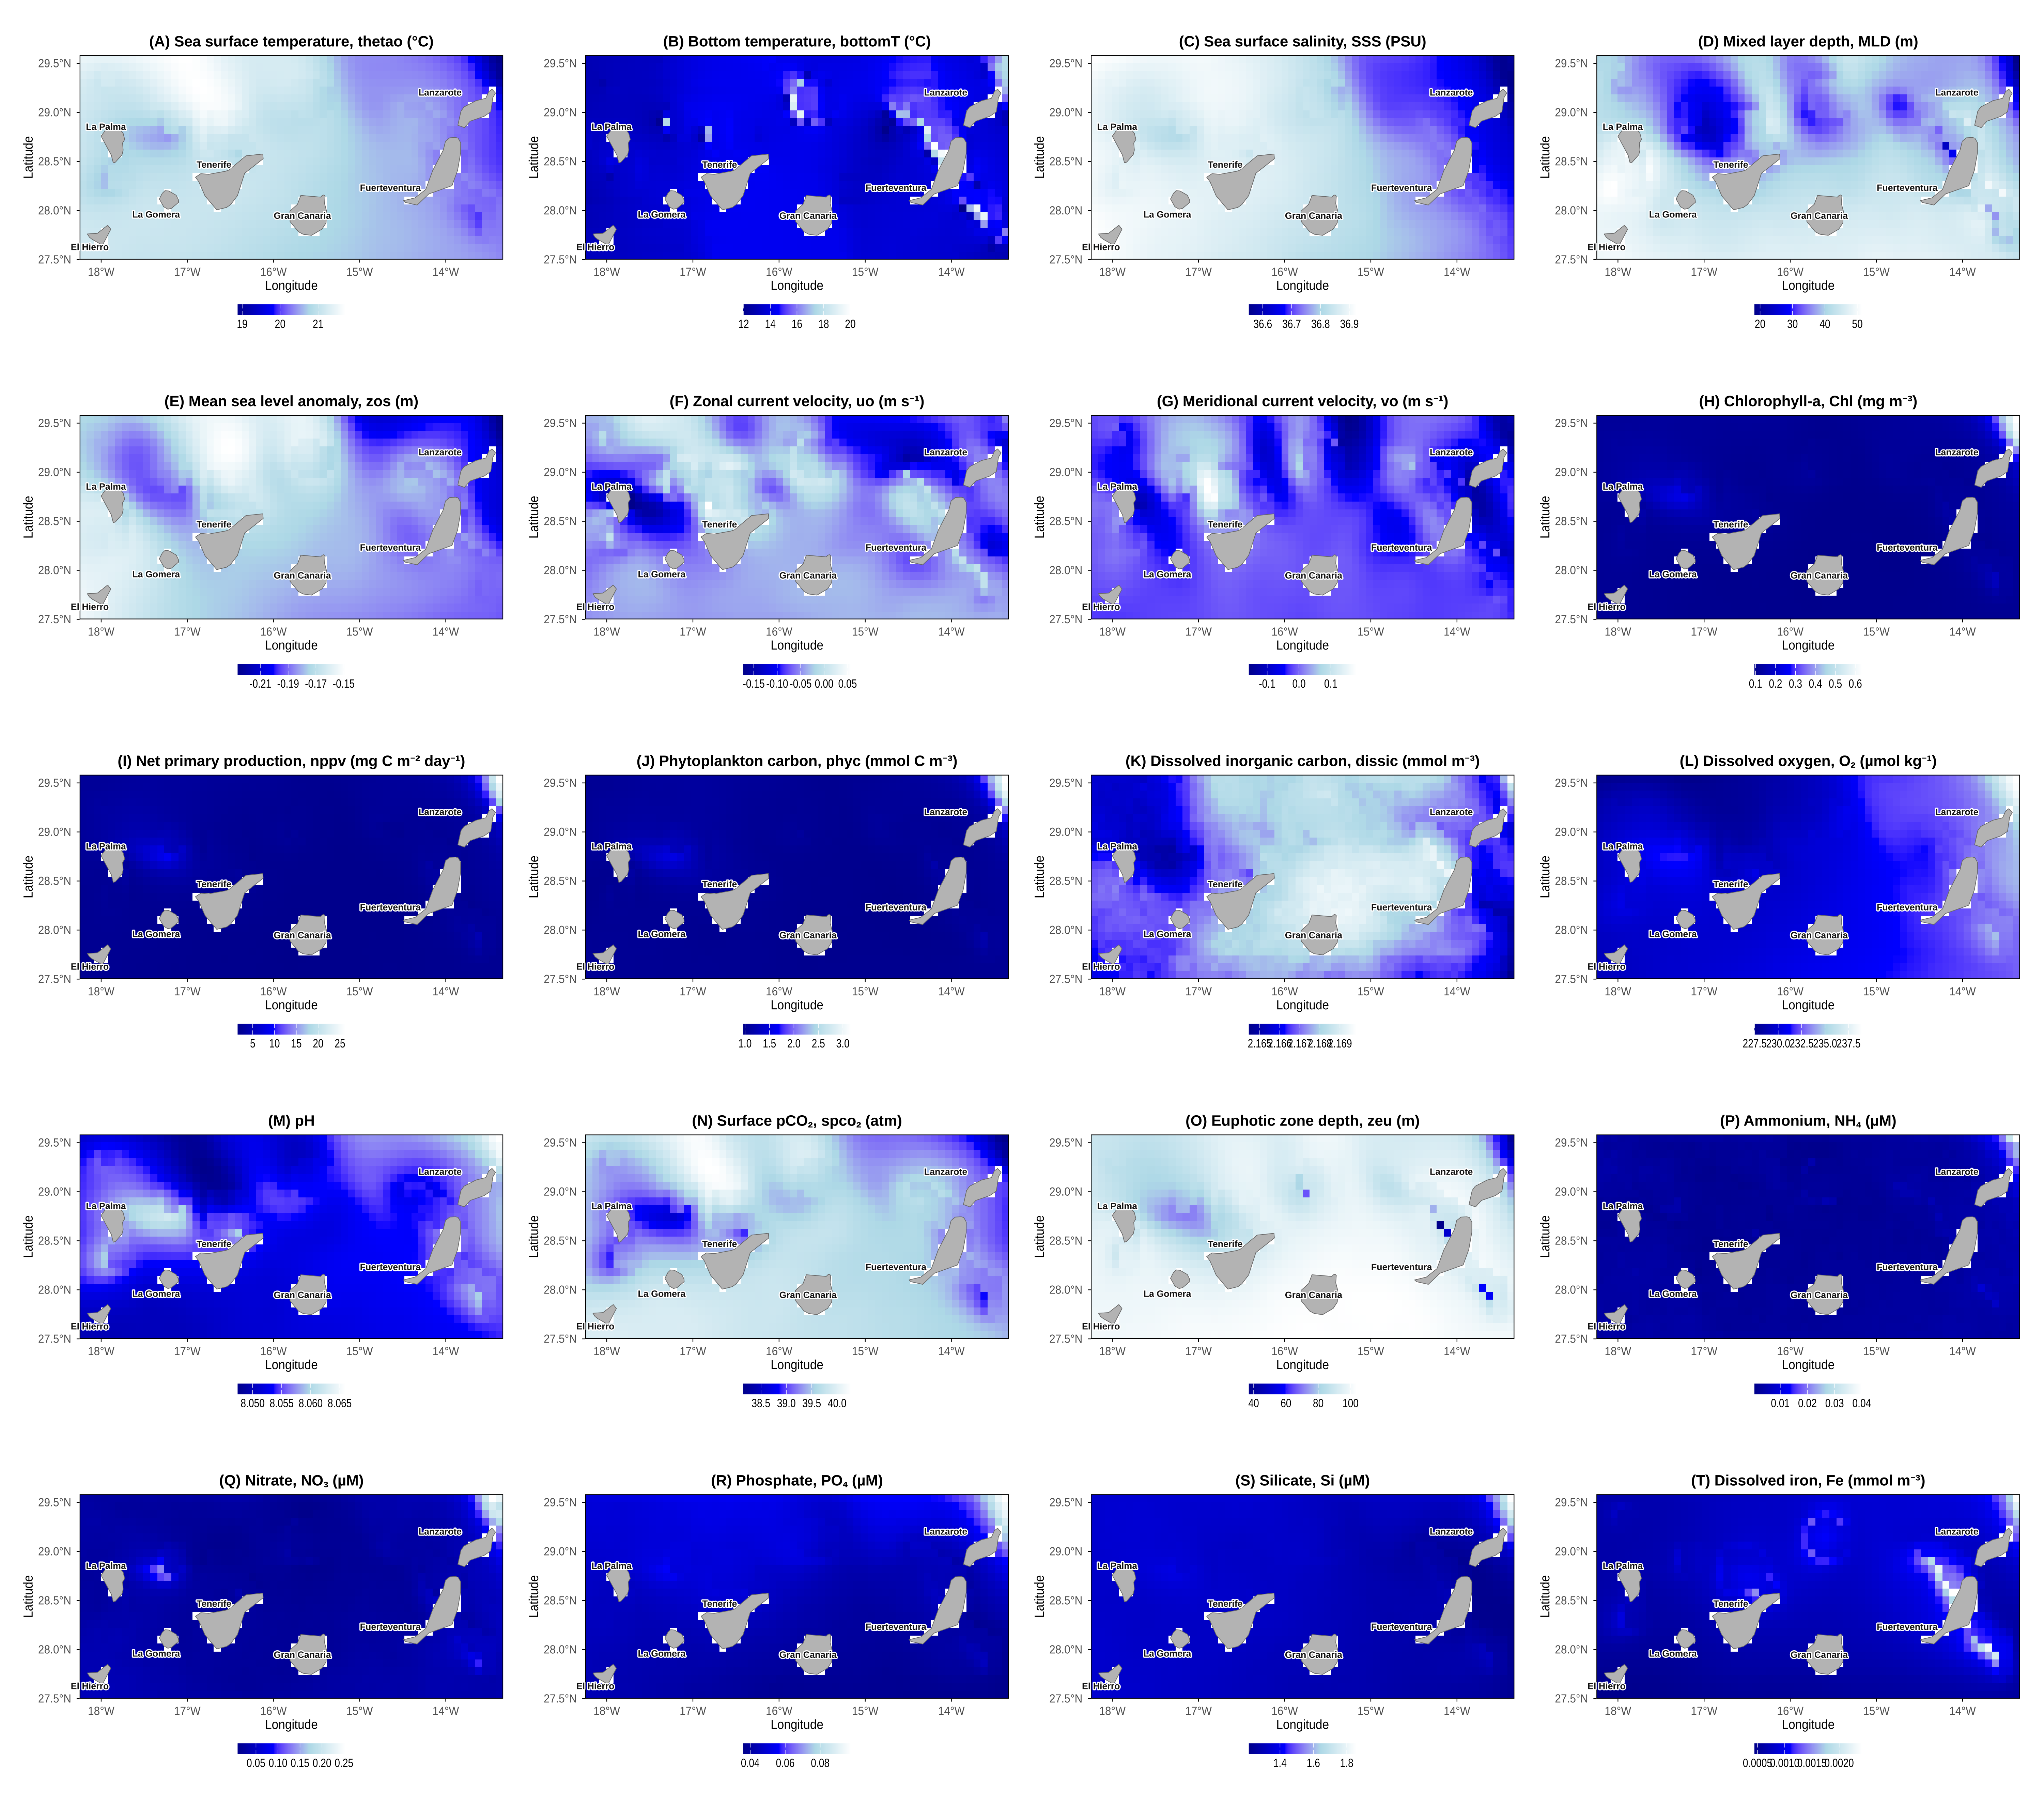
\includegraphics[width=\linewidth]{Figures/Fig 1.png}
\caption{Spatial distribution of physical and biogeochemical environmental variables across the Canary Islands archipelago, NE Atlantic. Panels show island-scale mean spatial fields of selected physical and biogeochemical variables derived from Copernicus Marine Environment Monitoring Service reanalysis products and averaged over the study period. The physical variables include A) Sea surface temperature (thetao, $ºC$), B) Bottom temperature (bottomT, $ºC$), C) Sea surface salinity (SSS, $PSU$), D) Mixed layer depth (MLD, $m$), E) Mean sea level anomaly (zos, $m$), and F) and G) Zonal and meridional current components (uo and vo, $m \cdot s^{-1}$). The biogeochemical variables include H) Chlorophyll-a concentration (Chl, $mg \cdot m^{-3}$), I) Net primary production of carbon (nppv, $mg C \cdot m^{-2} \cdot day^{-1}$), J) Phytoplankton biomass expressed as carbon (phyc, $mmolC \cdot m^{-3}$), K) Dissolved inorganic carbon (dissic, $mmol \cdot m^{-3}$), L) Dissolved oxygen ($O_{2}$, $µmol \cdot kg^{-1}$), M) Seawater $pH$ on the total scale, N) Surface partial pressure of $CO_{2}$ ($pCO_{2}$, $atm$), O) Euphotic zone depth (zeu, $m$),P) Ammonium ($NH_{4}$, $\mu M$), Q) Nitrate ($NO_{3}$, $\mu M$), R) Phosphate ($PO_{4}$, $\mu M$), S) Silicate ($Si$, $\mu M$), and T) Dissolved iron ($Fe$, $mmol \cdot m^{-3}$). Island names are displayed directly on the maps, and land areas are shown in grey.}
\label{fig:1}
\end{figure}

\begin{figure}[h]
\centering
\includegraphics[width=0.8\linewidth]{Figures/Fig 2.png}
\caption{\deleted{Satial}\added{Spatial} distribution of macroalgal species richness across the Canary Islands. Bars represent the total number of macroalgal species recorded for each island over the entire study period. Differences among islands reflect spatial heterogeneity in environmental conditions and variation in sampling intensity.}
\label{fig:2}
\end{figure}

\begin{figure}[h]
\centering
\includegraphics[width=0.8\linewidth]{Figures/Fig 3.png}
\caption{Spatial patterns of macroalgal beta diversity among the Canary Islands. Non-metric multidimensional scaling (NMDS) ordination based on Jaccard dissimilarity of macroalgal species composition among islands. Distances among points reflect compositional dissimilarity, with clustering indicating higher floristic similarity.}
\label{fig:3}
\end{figure}

\begin{figure}[h]
\centering
\includegraphics[width=0.8\linewidth]{Figures/Fig 4.png}
\caption{Decadal variability in macroalgal species richness across the Canary Islands. Bars show decadal averages of island-level species richness from the 1990s to the 2020s, illustrating long-term temporal changes in macroalgal diversity across the archipelago.}
\label{fig:4}
\end{figure}

\begin{figure}[h]
\centering
\includegraphics[width=0.8\linewidth]{Figures/Fig 5.png}
\caption{Seasonal and inter-decadal variability of selected environmental variables. Lines represent mean monthly values averaged by decade for physical and biogeochemical variables derived from Copernicus reanalysis products. The figure highlights seasonal cycles and changes in their amplitude across decades.}
\label{fig:5}
\end{figure}

\FloatBarrier

\subsection{Tables}
\begin{table}[width=\linewidth,cols=2,pos=!htbp]
\caption{Taxonomic breadth and temporal coverage of the macroalgal occurrence dataset used in this study. The table summarizes the number of taxa recorded at each hierarchical taxonomic level, the number of islands included, and the total temporal extent of the records.}
\small
\begin{tabular*}{\tblwidth}{@{} L R @{}}
\toprule
Level & Count \\
\midrule
Kingdoms & 2 \\
Phyla & 4 \\
Classes & 14 \\
Orders & 49 \\
Families & 111 \\
Genera & 289 \\
Species & 573 \\
Islands & 7 \\
Years & 30 \\
\bottomrule
\end{tabular*}
\label{tab:1}
\end{table}

\begin{table}[width=\linewidth,cols=2,pos=!htbp]
\caption{Number of macroalgal occurrence records compiled per year between 1992 and 2021. The table illustrates the uneven temporal distribution of sampling effort across the study period.}
\small
\begin{tabular*}{\tblwidth}{@{} L R @{}}
\toprule
Year & Count \\
\midrule
1992 & 714 \\
1993 & 1615 \\
1994 & 463 \\
1995 & 248 \\
1996 & 2602 \\
1997 & 317 \\
1998 & 1396 \\
1999 & 749 \\
2000 & 846 \\
2001 & 2221 \\
2002 & 1504 \\
2003 & 1589 \\
2004 & 707 \\
2005 & 29986 \\
2006 & 290 \\
2007 & 426 \\
2008 & 7319 \\
2009 & 306 \\
2010 & 59 \\
2011 & 2797 \\
2012 & 343 \\
2013 & 163 \\
2014 & 6021 \\
2015 & 581 \\
2016 & 62 \\
2017 & 108 \\
2018 & 418 \\
2019 & 55 \\
2020 & 43 \\
2021 & 442 \\
\bottomrule
\end{tabular*}
\label{tab:2}
\end{table}


\begin{table}[width=\linewidth,cols=2,pos=!htbp]
\caption{Distribution of macroalgal occurrence records among islands in the Canary Islands archipelago. Values reflect spatial differences in sampling intensity across islands.}
\small
\begin{tabular*}{\tblwidth}{@{} L R @{}}
\toprule
Island & Counts \\
\midrule
Lanzarote & 20756 \\
Tenerife & 8822 \\
Gran Canaria & 8794 \\
La Palma & 8566 \\
El Hierro & 8343 \\
Fuerteventura & 7515 \\
La Gomera & 1594 \\
\bottomrule
\end{tabular*}
\label{tab:3}
\end{table}

\begin{table}[width=\linewidth,cols=10,pos=!htbp]
\caption{Summary statistics of physical and biogeochemical environmental variables extracted from Copernicus Marine Environment Monitoring Service reanalysis products and matched to macroalgal records. Values correspond to monthly data aggregated across the study period \cite{CMEMS_BGC_IBI2024, CMEMS_PHY_IBI2024}.}
\small
\begin{tabular*}{\tblwidth}{@{} LLLLLLLLL R @{}}
\toprule
Variable & Analysis name & Unit & Min & Q1 & Median & Mean & Q3 & Max & NA \\
\midrule
Sea Surface Temperature & thetao & $^\circ$C & 18.92 & 20.31 & 20.47 & 20.63 & 20.70 & 23.35 & 1846 \\
Bottom temperature & bottomT & $^\circ$C & 12.04 & 13.67 & 13.92 & 13.82 & 14.01 & 15.36 & 9157 \\
Mixed Layer Depth & MLD & m & 10.80 & 16.40 & 17.80 & 19.08 & 21.50 & 37.20 & 1846 \\
Sea Surface Salinity & SSS & PSU & 36.25 & 36.55 & 36.59 & 36.69 & 36.85 & 37.22 & 1846 \\
Zonal current component & uo & m\,s$^{-1}$ & -0.2820 & -0.1230 & -0.1000 & -0.0983 & -0.0770 & 0.1600 & 1846 \\
Meridional current component & vo & m\,s$^{-1}$ & -0.2680 & -0.1410 & -0.1100 & -0.1002 & -0.0630 & 0.2560 & 1846 \\
Mean sea level anomaly & zos & m & -0.2940 & -0.2170 & -0.2100 & -0.2052 & -0.1930 & -0.0800 & 1846 \\
Chlorophyll-a concentration & Chl & mg\,m$^{-3}$ & 0.050 & 0.070 & 0.070 & 0.087 & 0.080 & 0.280 & 1846 \\
Dissolved inorganic carbon & dissic & mmol\,m$^{-3}$ & 2.140 & 2.170 & 2.170 & 2.172 & 2.180 & 2.190 & 1846 \\
Mole concentration of iron & fe & mmol\,m$^{-3}$ & 0.0003 & 0.0007 & 0.0007 & 0.0008 & 0.0009 & 0.0016 & 1846 \\
Mole concentration of ammonium & nh4 & $\mu$M & 0.0 & 0.0 & 0.0 & 0.0 & 0.0 & 0.1 & 1846 \\
Mole concentration of nitrate & no3 & $\mu$M & 0.0000 & 0.0000 & 0.0000 & 0.0006 & 0.0000 & 0.1000 & 1846 \\
Net primary production of carbon & nppv & mg\,C\,m$^{-2}$\,day$^{-1}$ & 0.000 & 1.000 & 1.000 & 1.779 & 1.000 & 20.000 & 1846 \\
Mole concentration of dissolved oxygen & o2 & $\mu$mol\,kg$^{-1}$ & 224.0 & 233.0 & 234.0 & 233.6 & 235.0 & 242.0 & 1846 \\
Sea water pH (total scale) & ph & -- & 8.011 & 8.048 & 8.050 & 8.050 & 8.052 & 8.074 & 1846 \\
Phytoplankton (as carbon) & phyc & mmol\,C\,m$^{-3}$ & 0.8000 & 0.9000 & 1.0000 & 0.9952 & 1.0000 & 1.7000 & 1846 \\
Mole concentration of phosphate & po4 & $\mu$M & 0.0300 & 0.0400 & 0.0400 & 0.0471 & 0.0500 & 0.1100 & 1846 \\
Mole concentration of silicate & si & $\mu$M & 0.700 & 1.200 & 1.300 & 1.284 & 1.300 & 1.900 & 1846 \\
Surface partial pressure of CO$_2$ & spco2 & atm & 37.30 & 39.60 & 40.00 & 39.96 & 40.22 & 44.38 & 1846 \\
Euphotic zone depth & zeu & m & 61.60 & 89.70 & 92.40 & 93.08 & 96.50 & 135.60 & 1846 \\
\bottomrule
\end{tabular*}
\label{tab:4}
\end{table}



\begin{table}[width=\linewidth,cols=5,pos=!htbp]
\caption{Results of multiple linear regression models relating macroalgal species richness (S) and Shannon diversity (H') to selected environmental variables. Estimates, standard errors, test statistics, and p-values are reported. Significant predictors are highlighted.}
\small
\begin{tabular*}{\tblwidth}{@{} LLLL R @{}}
\toprule
\textbf{Term} & \textbf{Estimate} & \textbf{Std. Error} & \textbf{t value} & \textbf{p value} \\
\midrule
\multicolumn{5}{l}{\textbf{Richness (S)}} \\
(Intercept)    & -2841.00 & 849.00    & -3.35 & \textbf{0.00088} \\
\deleted{thethao\_mean}\added{thetao\_mean}      & 35.80    & 8.67      & 4.13  & \textbf{0.00004} \\
bottomT\_mean & 4.28      & 2.74      & 1.56  & 0.119 \\
uo\_mean       & 169.00    & 25.80     & 6.56  & \textbf{1.45e-10} \\
vo\_mean       & -118.00   & 29.90     & -3.95 & \textbf{0.00009} \\
zos\_mean      & 243.00    & 67.80     & 3.58  & \textbf{0.00039} \\
dissic\_mean   & 857.00    & 257.00    & 3.33  & \textbf{0.00092} \\
fe\_mean       & -22648.00& 8278.00   & -2.74 & \textbf{0.00646} \\
nppv\_mean     & 1.64      & 0.94      & 1.74  & 0.0828 \\
o2\_mean       & 3.60      & 1.71      & 2.11  & \textbf{0.0354} \\
phyc\_mean     & 47.80     & 13.90     & 3.44  & \textbf{0.00063} \\
po4\_mean      & -259.00   & 153.00    & -1.69 & 0.0914 \\
spco2\_mean    & -14.50    & 2.87      & -5.04 & \textbf{6.68e-07} \\
zeu\_mean      & -0.23     & 0.16      & -1.42 & 0.155 \\
\midrule
\multicolumn{5}{l}{\textbf{Shannon (H')}} \\
(Intercept)    & -91.30    & 25.80     & -3.53 & \textbf{0.00045} \\
\deleted{thethao\_mean}\added{thetao\_mean}  & 1.01      & 0.15      & 6.73  & \textbf{5.12e-11} \\
bottomT\_mean  & 0.26      & 0.14      & 1.89  & 0.0590 \\
uo\_mean       & 7.50      & 1.34      & 5.59  & \textbf{3.90e-08} \\
vo\_mean       & -3.41     & 1.51      & -2.25 & \textbf{0.0248} \\
zos\_mean      & 8.38      & 3.43      & 2.44  & \textbf{0.0150} \\
chl\_mean      & -8.31     & 5.66      & -1.47 & 0.143 \\
dissic\_mean   & 47.80     & 12.20     & 3.92  & \textbf{0.00010} \\
phyc\_mean     & 2.97      & 1.20      & 2.48  & \textbf{0.0135} \\
po4\_mean      & -20.80    & 7.51      & -2.76 & \textbf{0.00595} \\
si\_mean       & 0.95      & 0.47      & 2.02  & \textbf{0.0436} \\
spco2\_mean    & -0.84     & 0.14      & -6.22 & \textbf{1.16e-09} \\
zeu\_mean      & -0.02     & 0.01      & -2.70 & \textbf{0.00722} \\
\bottomrule
\end{tabular*}
\label{tab:5}
\end{table}


\begin{table}[width=.9\linewidth,cols=4,pos=!htbp]
\caption{Principal component analysis summary. Eigenvalues, proportion of variance explained, and cumulative variance for each principal component derived from the environmental variables used in the analysis.}
\small
\begin{tabular*}{\tblwidth}{@{} LLL R @{}}
\toprule
\textbf{Component} & \textbf{Standard deviation} & \textbf{Proportion of Variance} & \textbf{Cumulative Proportion} \\
\midrule
PC1  & 2.5116 & 0.31540 & 0.31540 \\
PC2  & 1.7433 & 0.15200 & 0.46740 \\
PC3  & 1.6886 & 0.14260 & 0.60990 \\
PC4  & 1.4376 & 0.10330 & 0.71330 \\
PC5  & 1.08115 & 0.05844 & 0.77171 \\
PC6  & 1.03818 & 0.05389 & 0.82560 \\
PC7  & 0.94352 & 0.04451 & 0.87012 \\
PC8  & 0.88598 & 0.03925 & 0.90936 \\
PC9  & 0.68537 & 0.02349 & 0.93285 \\
PC10 & 0.61112 & 0.01867 & 0.95152 \\
PC11 & 0.51618 & 0.01332 & 0.96485 \\
PC12 & 0.47498 & 0.01128 & 0.97613 \\
PC13 & 0.40112 & 0.00804 & 0.98417 \\
PC14 & 0.35934 & 0.00646 & 0.99063 \\
PC15 & 0.30186 & 0.00456 & 0.99518 \\
PC16 & 0.26113 & 0.00341 & 0.99859 \\
PC17 & 0.14010 & 0.00098 & 0.99957 \\
PC18 & 0.08751 & 0.00038 & 0.99996 \\
PC19 & 0.02950 & 0.00004 & 1.00000 \\
PC20 & 4.285e-16 & 0.00000 & 1.00000 \\
\bottomrule
\end{tabular*}
\label{tab:6}
\end{table}


\begin{table}[!htbp]
\caption{PCA loadings of environmental variables: Loadings of environmental variables on principal components derived from the principal component analysis, indicating the contribution of each variable to the main environmental gradients.}
\centering
\scriptsize
\setlength{\tabcolsep}{2pt}
\renewcommand{\arraystretch}{1.1}
\makebox[\textwidth][c]{%
\begin{tabular}{lrrrrrrrrrrrrrrrrrrr}
\toprule
\textbf{Variable} & \textbf{PC1} & \textbf{PC2} & \textbf{PC3} & \textbf{PC4} & \textbf{PC5} & \textbf{PC6} & \textbf{PC7} & \textbf{PC8} & \textbf{PC9} & \textbf{PC10} & \textbf{PC11} & \textbf{PC12} & \textbf{PC13} & \textbf{PC14} & \textbf{PC15} & \textbf{PC16} & \textbf{PC17} & \textbf{PC18} & \textbf{PC19} \\
\midrule
s(\deleted{thethao\_mean}\added{thetao\_mean})      &  0.351 & -0.348 & -0.096 &  0.117 &  0.112 &  0.210 &  0.078 &  0.085 & -0.041 &  0.097 & -0.081 & -0.075 &  0.186 & -0.051 & -0.144 & -0.283 & -0.036 & -0.011 & -0.707 \\
s(bottomT\_mean)  & -0.075 &  0.052 &  0.048 & -0.090 &  0.483 & -0.351 &  0.380 &  0.302 &  0.111 & -0.040 & -0.072 &  0.522 &  0.286 &  0.064 &  0.043 & -0.083 &  0.042 & -0.021 &  0.000 \\
s(mlotst\_mean)   &  0.125 & -0.029 &  0.185 &  0.136 &  0.310 & -0.146 &  0.352 & -0.660 & -0.139 & -0.251 &  0.302 & -0.194 &  0.016 &  0.171 & -0.109 &  0.034 & -0.025 & -0.025 &  0.000 \\
s(so\_mean)       &  0.151 & -0.020 &  0.134 & -0.261 & -0.488 &  0.283 &  0.153 & -0.112 & -0.121 & -0.092 & -0.028 &  0.320 &  0.428 &  0.433 & -0.009 &  0.195 &  0.028 &  0.039 &  0.000 \\
s(uo\_mean)       &  0.132 &  0.030 &  0.338 &  0.261 & -0.230 & -0.174 &  0.059 &  0.470 & -0.008 & -0.192 &  0.512 & -0.247 &  0.280 & -0.182 &  0.076 &  0.098 & -0.058 &  0.026 &  0.000 \\
s(vo\_mean)       &  0.162 &  0.135 &  0.288 &  0.298 & -0.259 & -0.144 &  0.328 &  0.143 & -0.018 & -0.157 & -0.512 &  0.004 & -0.367 &  0.036 & -0.377 &  0.019 &  0.037 & -0.028 &  0.000 \\
s(zos\_mean)      &  0.223 &  0.077 &  0.037 & -0.501 &  0.093 & -0.217 & -0.164 &  0.050 &  0.020 &  0.220 &  0.136 & -0.084 &  0.040 & -0.109 & -0.668 &  0.258 & -0.064 & -0.037 &  0.000 \\
s(chl\_mean)      & -0.209 & -0.448 &  0.311 & -0.094 & -0.063 & -0.107 & -0.015 & -0.058 & -0.080 &  0.130 & -0.008 & -0.016 & -0.002 & -0.141 & -0.006 &  0.017 &  0.761 & -0.092 &  0.000 \\
s(dissic\_mean)   &  0.174 &  0.103 & -0.137 & -0.416 & -0.101 & -0.328 &  0.288 &  0.054 & -0.133 &  0.093 & -0.276 & -0.530 &  0.099 &  0.063 &  0.392 & -0.103 &  0.038 & -0.031 &  0.000 \\
s(fe\_mean)       &  0.180 & -0.106 &  0.029 &  0.295 & -0.074 & -0.475 & -0.416 & -0.107 &  0.368 &  0.208 & -0.075 & -0.020 &  0.132 &  0.495 &  0.043 & -0.044 &  0.015 & -0.025 &  0.000 \\
s(nppv\_mean)     &  0.238 &  0.360 & -0.337 & -0.006 & -0.043 &  0.080 &  0.060 &  0.162 & -0.013 & -0.051 &  0.383 &  0.058 & -0.260 &  0.292 & -0.095 & -0.303 &  0.495 & -0.104 &  0.000 \\
s(o2\_mean)       & -0.273 &  0.320 &  0.242 & -0.026 & -0.241 & -0.063 & -0.004 & -0.227 &  0.001 &  0.225 &  0.031 &  0.035 &  0.252 & -0.180 & -0.178 & -0.676 & -0.098 & -0.055 &  0.000 \\
s(ph\_mean)       &  0.379 &  0.074 &  0.345 & -0.116 &  0.075 &  0.060 & -0.188 & -0.051 & -0.083 &  0.026 &  0.000 &  0.219 & -0.178 & -0.125 &  0.301 & -0.025 & -0.112 & -0.682 &  0.000 \\
s(phyc\_mean)     &  0.193 &  0.413 & -0.073 &  0.142 &  0.145 &  0.144 & -0.184 & -0.165 &  0.229 & -0.256 & -0.293 & -0.100 &  0.437 & -0.316 & -0.007 &  0.172 &  0.360 & -0.012 &  0.000 \\
s(po4\_mean)      & -0.201 & -0.044 &  0.266 & -0.237 &  0.258 &  0.136 & -0.344 &  0.224 & -0.086 & -0.531 & -0.142 & -0.244 &  0.021 &  0.354 & -0.117 & -0.260 & -0.025 & -0.020 &  0.000 \\
s(si\_mean)       &  0.064 & -0.279 & -0.143 & -0.281 & -0.264 & -0.111 &  0.105 & -0.126 &  0.619 & -0.456 &  0.087 &  0.089 & -0.131 & -0.224 &  0.002 & -0.172 & -0.065 & -0.049 &  0.000 \\
s(spco2\_mean)    & -0.386 & -0.075 & -0.325 &  0.160 & -0.078 &  0.025 &  0.166 &  0.073 &  0.047 & -0.017 & -0.014 & -0.191 &  0.212 &  0.119 & -0.216 &  0.152 & -0.056 & -0.709 &  0.000 \\
s(zeu\_mean)      & -0.062 &  0.113 &  0.344 & -0.074 &  0.176 &  0.421 &  0.268 &  0.078 &  0.582 &  0.345 &  0.052 & -0.245 & -0.084 &  0.189 &  0.060 &  0.080 &  0.017 &  0.013 &  0.000 \\
\bottomrule
\end{tabular}}
\label{tab:7}
\end{table}
\FloatBarrier

\section{Annex I: Supplementary Material}
\added{Supplementary tables are numbered independently from the main manuscript tables.}
\setcounter{table}{0}
\renewcommand{\thetable}{S\arabic{table}}
%Tablas: 3,7,8,9,10,11,12,13,14,15,17,18

\begin{table}[width=\linewidth,cols=2,pos=!htbp]
\caption{Most frequently recorded macroalgal species in the dataset. The table lists the fifteen species with the highest number of occurrence records, indicating their relative representation across islands and years.}
\small
\begin{tabular*}{\tblwidth}{@{} L R @{}}
\toprule
Species & Count \\
\midrule
\textit{Gongolaria abiesmarina} & 3874 \\
\textit{Dunaliella salina} & 1704 \\
\textit{Gelidium canariense} & 1515 \\
\textit{Lobophora variegata} & 1481 \\
\textit{Caulerpa prolifera} & 1475 \\
\textit{Alsidium corallinum} & 1341 \\
\textit{Padina pavonica} & 1334 \\
\textit{Fucus spiralis} & 1332 \\
\textit{Caulerpa racemosa} & 1258 \\
\textit{Lophocladia trichoclados} & 1168 \\
\textit{Halopteris scoparia} & 1112 \\
\textit{Caulerpa webbiana} & 1088 \\
\textit{Jania pedunculata} & 1061 \\
\textit{Corallina ferreyrae} & 1056 \\
\textit{Cystoseira compressa} & 1014 \\
\bottomrule
\end{tabular*}
\label{tab:8}
\end{table}

\begin{table}[width=\linewidth,cols=5,pos=!htbp]
\caption{Summary of generalized additive models (GAMs) fitted to macroalgal species richness (S) and Shannon diversity (H'), including estimated degrees of freedom, test statistics, and p-values for each smooth term.}
\small
\begin{tabular*}{\tblwidth}{@{} LLLLL @{}}
\toprule
\textbf{Smooth term} & \textbf{edf} & \textbf{Ref.df} & \textbf{F} & \textbf{p value} \\
\midrule
\multicolumn{5}{l}{\textbf{Richness (S)}} \\
s(\deleted{\deleted{thethao\_mean}\added{thetao\_mean}}\added{thetao\_mean})      & 2.82 & 9 & 0.32  & \textbf{0.00062} \\
s(bottomT\_mean) & 5.41 & 9 & 1.76  & \textbf{0.00333} \\
s(mlotst\_mean)   & 6.14 & 9 & 2.90  & \textbf{4.69e-05} \\
s(so\_mean)       & 4.71 & 9 & 0.83  & 0.0866 \\
s(uo\_mean)       & 8.78 & 9 & 2.81  & \textbf{0.00141} \\
s(vo\_mean)       & 0.10 & 9 & 0.01  & 0.234 \\
s(zos\_mean)      & 8.26 & 9 & 3.14  & \textbf{0.00016} \\
s(chl\_mean)      & 5.83 & 9 & 2.84  & \textbf{1.06e-05} \\
s(dissic\_mean)   & 3.26 & 9 & 0.57  & 0.124 \\
s(fe\_mean)       & 3.46 & 9 & 0.96  & \textbf{0.0191} \\
s(nppv\_mean)     & 5.26 & 9 & 3.07  & \textbf{3.42e-06} \\
s(o2\_mean)       & 2.81 & 9 & 1.17  & \textbf{0.00245} \\
s(ph\_mean)       & 7.43 & 9 & 3.77  & \textbf{1.30e-06} \\
s(phyc\_mean)     & 4.62 & 9 & 1.31  & \textbf{0.0101} \\
s(po4\_mean)      & 3.99 & 9 & 1.24  & \textbf{0.00840} \\
s(si\_mean)       & 4.85 & 9 & 3.14  & \textbf{1.99e-06} \\
s(spco2\_mean)    & 7.95 & 9 & 3.86  & \textbf{1.10e-06} \\
s(zeu\_mean)      & 0.00 & 9 & 0.00  & 0.882 \\
\midrule
\multicolumn{5}{l}{\textbf{Shannon (H')}} \\
s(\deleted{thethao\_mean}\added{thetao\_mean})      & 4.08 & 9 & 0.21  & \textbf{0.00239} \\
s(bottomT\_mean) & 3.96 & 9 & 1.99  & \textbf{0.00029} \\
s(mlotst\_mean)   & 5.18 & 9 & 1.66  & \textbf{0.00487} \\
s(so\_mean)       & 0.00 & 9 & 0.00  & 0.811 \\
s(uo\_mean)       & 0.18 & 9 & 0.04  & 0.168 \\
s(vo\_mean)       & 0.00 & 9 & 0.00  & 0.373 \\
s(zos\_mean)      & 7.81 & 9 & 2.13  & \textbf{0.00555} \\
s(chl\_mean)      & 6.31 & 9 & 3.30  & \textbf{1.84e-06} \\
s(dissic\_mean)   & 2.52 & 9 & 0.42  & 0.158 \\
s(fe\_mean)       & 3.42 & 9 & 1.18  & \textbf{0.00699} \\
s(nppv\_mean)     & 6.30 & 9 & 2.89  & \textbf{3.88e-05} \\
s(o2\_mean)       & 7.69 & 9 & 5.09  & \textbf{<2e-16} \\
s(ph\_mean)       & 5.25 & 9 & 1.89  & \textbf{0.00050} \\
s(phyc\_mean)     & 2.79 & 9 & 0.90  & \textbf{0.0121} \\
s(po4\_mean)      & 5.99 & 9 & 2.55  & \textbf{0.00022} \\
s(si\_mean)       & 4.58 & 9 & 3.12  & \textbf{1.74e-06} \\
s(spco2\_mean)    & 7.71 & 9 & 2.69  & \textbf{2.73e-05} \\
s(zeu\_mean)      & 5.51 & 9 & 1.72  & \textbf{0.00375} \\
\bottomrule
\end{tabular*}
\label{tab:9}
\end{table}

\begin{table}[width=\linewidth,cols=5,pos=!htbp]
\caption{Results of the generalized additive model fitted to macroalgal species richness (S) using a Poisson error distribution. Estimated degrees of freedom, test statistics, and p-values are reported for each environmental predictor.}
\small
\begin{tabular*}{\tblwidth}{@{} LLLLL @{}}
\toprule
\textbf{Smooth term} & \textbf{edf} & \textbf{Ref.df} & \textbf{Chi.sq} & \textbf{p value} \\
\midrule
s(\deleted{thethao\_mean}\added{thetao\_mean})      & 4.50 & 9 & 0.004  & \textbf{$<2 \times 10^{-16}$} \\
s(bottomT\_mean) & 7.76 & 9 & 245.93 & \textbf{$<2 \times 10^{-16}$} \\
s(mlotst\_mean)   & 8.22 & 9 & 203.46 & \textbf{$<2 \times 10^{-16}$} \\
s(so\_mean)       & 8.41 & 9 & 76.22  & \textbf{$<2 \times 10^{-16}$} \\
s(uo\_mean)       & 9.00 & 9 & 168.76 & \textbf{$<2 \times 10^{-16}$} \\
s(vo\_mean)       & 7.02 & 9 & 79.56  & \textbf{$<2 \times 10^{-16}$} \\
s(zos\_mean)      & 8.64 & 9 & 136.16 & \textbf{$<2 \times 10^{-16}$} \\
s(chl\_mean)      & 8.93 & 9 & 114.34 & \textbf{$<2 \times 10^{-16}$} \\
s(dissic\_mean)   & 8.84 & 9 & 120.80 & \textbf{$<2 \times 10^{-16}$} \\
s(fe\_mean)       & 8.87 & 9 & 103.57 & \textbf{$<2 \times 10^{-16}$} \\
s(nppv\_mean)     & 7.78 & 9 & 87.99  & \textbf{$<2 \times 10^{-16}$} \\
s(o2\_mean)       & 7.16 & 9 & 170.49 & \textbf{$<2 \times 10^{-16}$} \\
s(ph\_mean)       & 8.52 & 9 & 250.35 & \textbf{$<2 \times 10^{-16}$} \\
s(phyc\_mean)     & 9.00 & 9 & 196.73 & \textbf{$<2 \times 10^{-16}$} \\
s(po4\_mean)      & 8.83 & 9 & 110.62 & \textbf{$<2 \times 10^{-16}$} \\
s(si\_mean)       & 7.93 & 9 & 109.83 & \textbf{$<2 \times 10^{-16}$} \\
s(spco2\_mean)    & 9.00 & 9 & 294.07 & \textbf{$<2 \times 10^{-16}$} \\
s(zeu\_mean)      & 8.89 & 9 & 86.45  & \textbf{$<2 \times 10^{-16}$} \\
\bottomrule
\end{tabular*}
\label{tab:10}
\end{table}
\FloatBarrier

\begin{table}[width=\linewidth,cols=5,pos=!htbp]
\caption{Results of the generalized additive model fitted to Shannon diversity (H') using a Gaussian error distribution. Estimated degrees of freedom, F-statistics, and p-values are reported for each smooth term.}
\begin{tabular*}{\tblwidth}{@{} LLLLL @{}}
\toprule
\textbf{Smooth term} & \textbf{edf} & \textbf{Ref.df} & \textbf{F} & \textbf{p value} \\
\midrule
s(\deleted{thethao\_mean}\added{thetao\_mean})      & 4.08 & 9 & 0.21 & \textbf{0.0024} \\
s(bottomT\_mean) & 3.96 & 9 & 1.99 & \textbf{0.00029} \\
s(mlotst\_mean)   & 5.18 & 9 & 1.66 & \textbf{0.0049} \\
s(so\_mean)       & 0.00 & 9 & 0.00 & 0.811 \\
s(uo\_mean)       & 0.18 & 9 & 0.04 & 0.168 \\
s(vo\_mean)       & 0.00 & 9 & 0.00 & 0.373 \\
s(zos\_mean)      & 7.81 & 9 & 2.13 & \textbf{0.0055} \\
s(chl\_mean)      & 6.31 & 9 & 3.30 & \textbf{1.8e-06} \\
s(dissic\_mean)   & 2.52 & 9 & 0.42 & 0.158 \\
s(fe\_mean)       & 3.42 & 9 & 1.18 & \textbf{0.0070} \\
s(nppv\_mean)     & 6.30 & 9 & 2.89 & \textbf{3.9e-05} \\
s(o2\_mean)       & 7.69 & 9 & 5.09 & \textbf{$<2 \times 10^{-16}$} \\
s(ph\_mean)       & 5.25 & 9 & 1.89 & \textbf{0.00050} \\
s(phyc\_mean)     & 2.79 & 9 & 0.90 & \textbf{0.012} \\
s(po4\_mean)      & 5.99 & 9 & 2.55 & \textbf{0.00022} \\
s(si\_mean)       & 4.58 & 9 & 3.12 & \textbf{1.7e-06} \\
s(spco2\_mean)    & 7.71 & 9 & 2.69 & \textbf{2.7e-05} \\
s(zeu\_mean)      & 5.51 & 9 & 1.72 & \textbf{0.0038} \\
\bottomrule
\end{tabular*}
\label{tab:11}
\end{table}

\begin{table}[width=\linewidth,cols=4,pos=!htbp]
\caption{Spectral and spatial resolution specifications for Sentinel-2 and Landsat 8 sensors used for ancillary remote-sensing analyses.}
\small
\begin{tabular*}{\tblwidth}{@{} LLLL @{}}
\toprule
\multicolumn{2}{l}{\textbf{Sentinel-2 (5-day revisit)}} & \multicolumn{2}{l}{\textbf{Landsat 8 (16-day revisit)}} \\
\midrule
Band & Wavelength (nm) / spatial resolution (m) & Band & Wavelength (nm) / spatial resolution (m) \\
\midrule
1 & 443/60 & 1 & 443/30 \\
2 & 490/10 & 2 & 483/30 \\
3 & 560/10 & 3 & 561/30 \\
4 & 665/10 & 4 & 655/30 \\
5 & 704/20 & 5 & 865/30 \\
6 & 740/20 & 8 & 590/15 \\
7 & 783/20 & -- & -- \\
8 & 842/10 & -- & -- \\
8A & 865/20 & -- & -- \\
\bottomrule
\end{tabular*}
\label{tab:12}
\end{table}

\begin{table}[width=\linewidth,cols=6,pos=!htbp]
\caption{Spectral characteristics and spatial resolution of Sentinel-2 bands.}
\small
\begin{tabular*}{\tblwidth}{@{} LLLLLL @{}}
\toprule
\textbf{Spectral region} & \textbf{Band} & \textbf{$\lambda_{S2A}$ (nm)} & \textbf{$\lambda_{S2B}$ (nm)} & \textbf{Bandwidth (nm)} & \textbf{Spatial resolution (m)} \\
\midrule
Coastal aerosol & B1 & 442.7 & 442.2 & 21--21 & 60 \\
Blue & B2 & 492.4 & 492.1 & 66--66 & 10 \\
Green & B3 & 559.8 & 559.0 & 36--36 & 10 \\
Red & B4 & 664.6 & 664.9 & 31--31 & 10 \\
Red-edge 1 & B5 & 704.1 & 703.8 & 15--16 & 20 \\
Red-edge 2 & B6 & 740.5 & 739.1 & 15--15 & 20 \\
Red-edge 3 & B7 & 782.8 & 779.7 & 20--20 & 20 \\
NIR & B8 & 832.8 & 832.9 & 106--106 & 10 \\
NIR narrow & B8A & 864.7 & 864.0 & 21--22 & 20 \\
\bottomrule
\end{tabular*}
\label{tab:13}
\end{table}

\begin{table}[width=.9\linewidth,cols=6,pos=!htbp]
\caption{Linear regression statistics of giant kelp for NDREB index (kelp canopy area) and tidal height}
\small
\begin{tabular*}{\tblwidth}{@{} LLLLLLL@{} }
\toprule
Season & Threshold &Slope & Intercept & R$^{2}$ & F-Statistic & n\\
\midrule
Summer  & dynamic & -0.84 $\pm$ 0.31 & 3.5 $\pm$ 0.57 & 0.06 & 7.32 & 119 \\
Autumn  & dynamic & -0.47 $\pm$ 0.24 & 2.53 $\pm$ 0.53 & 0.05 & 3.699 & 66 \\
Winter  & dynamic & -0.54 $\pm$ 0.1 & 1.82 $\pm$ 0.23 & 0.36 & 27.81 & 52 \\
Spring  & dynamic & -0.54 $\pm$ 0.23 & 2.56 $\pm$ 0.43 & 0.06 & 5.371 & 83 \\
Total  & dynamic & -0.84 $\pm$ 0.13 & 3.19 $\pm$ 0.25 & 0.12 & 45.18 & 320 \\
Summer  & >0 & -1.12 $\pm$ 0.33 & 3.58 $\pm$ 0.62 & 0.09 & 11.27 & 119 \\
Autumn  & >0 & -0.48 $\pm$ 0.26 & 1.98 $\pm$ 0.57 & 0.05 & 3.518 & 66 \\
Winter  & >0 & -0.31 $\pm$ 0.08 & 0.95 $\pm$ 0.17 & 0.25 & 16.82 & 52 \\
Spring  & >0 & -0.54 $\pm$ 0.31 & 2.27 $\pm$ 0.57 & 0.04 & 3.056 & 83 \\
Total  & >0 & -0.91 $\pm$ 0.14 & 2.92 $\pm$ 0.27 & 0.12 & 44.3 & 320 \\
\bottomrule
\end{tabular*}
\label{tab:14}
\end{table}

\begin{table}[width=.9\linewidth,cols=6,pos=!htbp]
\caption{Linear regression statistics of giant kelp for NDREB index (kelp canopy area) and NDTI index (turbidity)}
\small
\begin{tabular*}{\tblwidth}{@{} LLLLLLL@{} }
\toprule
Season & Threshold &Slope & Intercept & R$^{2}$ & F-Statistic & n\\
\midrule
Summer  & dynamic & -0.11 $\pm$ 0.55 & 1.93 $\pm$ 0.2 & 0.0003 & 0.04 & 119 \\
Autumn  & dynamic & 1.38 $\pm$ 0.47 & 2.32 $\pm$ 0.29 & 0.12 & 8.58 & 66 \\
Winter  & dynamic & -0.45 $\pm$ 0.32 & 0.4 $\pm$ 0.19 & 0.04 & 2.029 & 52 \\
Spring  & dynamic & 0.23 $\pm$ 0.55 & 1.64 $\pm$ 0.17 & 0.002 & 0.18 & 83 \\
Total  & dynamic & 0.93 $\pm$ 0.23 & 1.93 $\pm$ 0.11 & 0.05 & 15.55 & 320 \\
Summer  & >0 & 1.32 $\pm$ 0.59 & 1.98 $\pm$ 0.22 & 0.04 & 5.07 & 119 \\
Autumn  & >0 & 1.11 $\pm$ 0.52 & 1.58 $\pm$ 0.32 & 0.07 & 4.58 & 66 \\
Winter  & >0 & -0.53 $\pm$ 0.21 & -0.01 $\pm$ 0.12 & 0.12 & 6.51 & 52 \\
Spring  & >0 & 1.4 $\pm$ 0.7 & 1.68 $\pm$ 0.22 & 0.05 & 4.06 & 83 \\
Total  & >0 & 1.58 $\pm$ 0.25 & 1.79 $\pm$ 0.11 & 0.11 & 40.22 & 320 \\\bottomrule
\end{tabular*}
\label{tab:15}
\end{table}

\begin{table}[width=.9\linewidth,cols=4,pos=!htbp]
\caption{Results of the linear regression model between the seasonal time series area of \textit{M. pyrifera} (ha) and \textit{offshore} nutrients.}\label{nutrientoff}
\small
\begin{tabular*}{\tblwidth}{@{} LLLL@{} }
\toprule
Variable & F-Statistic & p-value & R$^{2}$ (Adj) \\
\midrule
Nitrate offshore & 0.176 & 0.686 & -0.101 \\
Nitrite offshore & 0.059 & 0.814 & -0.117 \\
Phosphate offshore & 0.497 & 0.501 & -0.059 \\
N:P offshore & 1.383 & 0.273 & 0.041 \\
Silicate offshore & 1.231 & 0.299 & 0.025 \\
\bottomrule
\end{tabular*}
\label{tab:16}
\end{table}

\begin{table}[width=.9\linewidth,cols=5,pos=!htbp]
\caption{GAM fitted to visualization subset. Generalized additive model for species richness (S) fitted to a reduced visualization subset of the data. Model performance metrics and smooth term statistics are reported.}
\small
\begin{tabular*}{\tblwidth}{@{} LLLLL @{}}
\toprule
\textbf{Smooth term} & \textbf{edf} & \textbf{Ref.df} & \textbf{Chi.sq} & \textbf{p value} \\
\midrule
s(\deleted{thethao\_mean}\added{thetao\_mean})      & 2.8000 & 9 &  3.302 & $<2 \times 10^{-16}$ \\
s(bottomT\_mean) & 9.0000 & 9 & 54.722 & $<2 \times 10^{-16}$ \\
s(mlotst\_mean)   & 9.0000 & 9 & 41.813 & $<2 \times 10^{-16}$ \\
s(so\_mean)       & 6.0019 & 9 & 17.781 & 8.73e-05 \\
s(uo\_mean)       & 8.7343 & 9 & 32.021 & $<2 \times 10^{-16}$ \\
s(vo\_mean)       & 8.8313 & 9 & 39.450 & $<2 \times 10^{-16}$ \\
s(zos\_mean)      & 8.6311 & 9 & 50.598 & $<2 \times 10^{-16}$ \\
s(chl\_mean)      & 1.2697 & 9 &  4.539 & 0.00606  \\
s(dissic\_mean)   & 0.9321 & 8 & 10.449 & 1.86e-05 \\
s(fe\_mean)       & 8.9929 & 9 & 55.055 & $<2 \times 10^{-16}$ \\
s(no3\_mean)      & 2.9999 & 3 &  4.619 & 0.06180  \\
s(nppv\_mean)     & 6.2908 & 9 & 29.497 & $<2 \times 10^{-16}$ \\
s(o2\_mean)       & 5.0230 & 9 & 20.658 & $<2 \times 10^{-16}$ \\
s(ph\_mean)       & 5.8639 & 9 & 27.064 & $<2 \times 10^{-16}$ \\
s(phyc\_mean)     & 7.1125 & 9 & 19.656 & 8.64e-05 \\
s(po4\_mean)      & 5.5078 & 9 & 22.559 & 4.30e-07 \\
s(si\_mean)       & 6.6748 & 9 & 45.417 & $<2 \times 10^{-16}$ \\
s(spco2\_mean)    & 7.5839 & 9 & 22.537 & $<2 \times 10^{-16}$ \\
s(zeu\_mean)      & 6.6533 & 9 & 39.218 & $<2 \times 10^{-16}$ \\
\bottomrule
\end{tabular*}
\label{tab:17}
\end{table}
\FloatBarrier


\begin{table}[width=.9\linewidth,cols=5,pos=!htbp]
\caption{Regional GAM for species richness (S). Generalized additive model results for S fitted at the regional scale. Estimated degrees of freedom, test statistics, and p-values are reported for each smooth term.}
\small
\begin{tabular*}{\tblwidth}{@{} LLLLL @{}}
\toprule
\textbf{Smooth term} & \textbf{edf} & \textbf{Ref.df} & \textbf{Chi.sq} & \textbf{p-value} \\
\midrule
s(\deleted{thethao\_mean}\added{thetao\_mean})      & 4.500 & 9 &   0.004 & $<2 \times 10^{-16}$ \\
s(bottomT\_mean) & 7.760 & 9 & 245.930 & $<2 \times 10^{-16}$ \\
s(mlotst\_mean)   & 8.224 & 9 & 203.457 & $<2 \times 10^{-16}$ \\
s(so\_mean)       & 8.407 & 9 &  76.222 & $<2 \times 10^{-16}$ \\
s(uo\_mean)       & 8.998 & 9 & 168.761 & $<2 \times 10^{-16}$ \\
s(vo\_mean)       & 7.020 & 9 &  79.559 & $<2 \times 10^{-16}$ \\
s(zos\_mean)      & 8.636 & 9 & 136.156 & $<2 \times 10^{-16}$ \\
s(chl\_mean)      & 8.934 & 9 & 114.340 & $<2 \times 10^{-16}$ \\
s(dissic\_mean)   & 8.844 & 9 & 120.795 & $<2 \times 10^{-16}$ \\
s(fe\_mean)       & 8.869 & 9 & 103.565 & $<2 \times 10^{-16}$ \\
s(nppv\_mean)     & 7.777 & 9 &  87.989 & $<2 \times 10^{-16}$ \\
s(o2\_mean)       & 7.157 & 9 & 170.490 & $<2 \times 10^{-16}$ \\
s(ph\_mean)       & 8.515 & 9 & 250.347 & $<2 \times 10^{-16}$ \\
s(phyc\_mean)     & 9.000 & 9 & 196.731 & $<2 \times 10^{-16}$ \\
s(po4\_mean)      & 8.825 & 9 & 110.617 & $<2 \times 10^{-16}$ \\
s(si\_mean)       & 7.927 & 9 & 109.826 & $<2 \times 10^{-16}$ \\
s(spco2\_mean)    & 9.000 & 9 & 294.070 & $<2 \times 10^{-16}$ \\
s(zeu\_mean)      & 8.893 & 9 &  86.448 & $<2 \times 10^{-16}$ \\
\bottomrule
\end{tabular*}
\label{tab:18}
\end{table}

\begin{table}[width=.9\linewidth,cols=5,pos=!htbp]
\caption{Regional GAM for Shannon diversity (H'): Generalized additive model results for H' fitted at the regional scale, reporting smooth term statistics and overall model performance.}
\small
\begin{tabular*}{\tblwidth}{@{} LLLLL @{}}
\toprule
\textbf{Smooth term} & \textbf{edf} & \textbf{Ref.df} & \textbf{F} & \textbf{p-value} \\
\midrule
s(\deleted{thethao\_mean}\added{thetao\_mean})      & 4.081 & 9 & 0.210 & 0.00239 ** \\
s(bottomT\_mean) & 3.963 & 9 & 1.994 & 0.00029 *** \\
s(mlotst\_mean)   & 5.177 & 9 & 1.661 & 0.00487 ** \\
s(so\_mean)       & 0.000 & 9 & 0.000 & 0.81118 \\
s(uo\_mean)       & 0.184 & 9 & 0.035 & 0.16844 \\
s(vo\_mean)       & 0.000 & 9 & 0.000 & 0.37314 \\
s(zos\_mean)      & 7.808 & 9 & 2.130 & 0.00555 ** \\
s(chl\_mean)      & 6.310 & 9 & 3.302 & 1.8e-06 *** \\
s(dissic\_mean)   & 2.516 & 9 & 0.416 & 0.15787 \\
s(fe\_mean)       & 3.421 & 9 & 1.176 & 0.00699 ** \\
s(nppv\_mean)     & 6.295 & 9 & 2.885 & 3.9e-05 *** \\
s(o2\_mean)       & 7.692 & 9 & 5.087 & $<2 \times 10^{-16}$ *** \\
s(ph\_mean)       & 5.254 & 9 & 1.892 & 0.00050 *** \\
s(phyc\_mean)     & 2.792 & 9 & 0.895 & 0.01212 * \\
s(po4\_mean)      & 5.991 & 9 & 2.545 & 0.00022 *** \\
s(si\_mean)       & 4.576 & 9 & 3.120 & 1.7e-06 *** \\
s(spco2\_mean)    & 7.709 & 9 & 2.687 & 2.7e-05 *** \\
s(zeu\_mean)      & 5.507 & 9 & 1.716 & 0.00375 ** \\
\bottomrule
\end{tabular*}
\label{tab:19}
\end{table}

\end{document}

